  \documentclass[12pt]{exam}
\usepackage{amsthm}
\usepackage{libertine}
\usepackage[utf8]{inputenc}
\usepackage[margin=1in]{geometry}
\usepackage{amsmath,amssymb}
\usepackage{multicol}
\usepackage[shortlabels]{enumitem}
\usepackage{siunitx}
\usepackage[T1]{fontenc}
\usepackage{cancel}
\usepackage{graphicx}
\usepackage{pgfplots}
\usepackage{listings}
\usepackage{tikz}
\usepackage{float}
\usepackage{url}

\pgfplotsset{width=10cm,compat=1.9}
\usepgfplotslibrary{external}
\tikzexternalize

\newcommand{\class}{Laboratorio Intermedio} % This is the name of the course 
\newcommand{\examnum}{Tarea Bibliografia} % This is the name of the assignment
\newcommand{\examdate}{\today} % This is the due date
\newcommand{\timelimit}{}



\begin{document}
\pagestyle{plain}
\thispagestyle{empty}

\noindent
\begin{tabular*}{\textwidth}{l @{\extracolsep{\fill}} r @{\extracolsep{6pt}} l}
	\textbf{\class} & \textbf{Nombre:} & \textit{Sergio Montoya Ramirez}\\ %Your name here instead, obviously 
	\textbf{\examnum} &&\textit{Angelica Lopez Duarte}\\
	\textbf{\examdate} &&
\end{tabular*}\\
\rule[2ex]{\textwidth}{2pt}
% ---

\section{}
\subsection{}
En primer lugar, ingresamos a google scholar y buscamos artículos de nuestro interés

\begin{figure}[H]
    \centering
    
\includegraphics[width=0.8\linewidth]{heidegger tecnica y ciencia.png}
    \label{}
\end{figure}

\begin{figure}[H]
    \centering
    
\includegraphics[width=0.8\linewidth]{biofisica .png}
    \label{}
\end{figure}

\subsection{}
Luego, para cada artículo seleccionamos la opción de citado por y accedemos a los documentos en los que han sido citados, como se muestra a continuación 

Para el primer artículo
\begin{figure}[H]
    \centering
    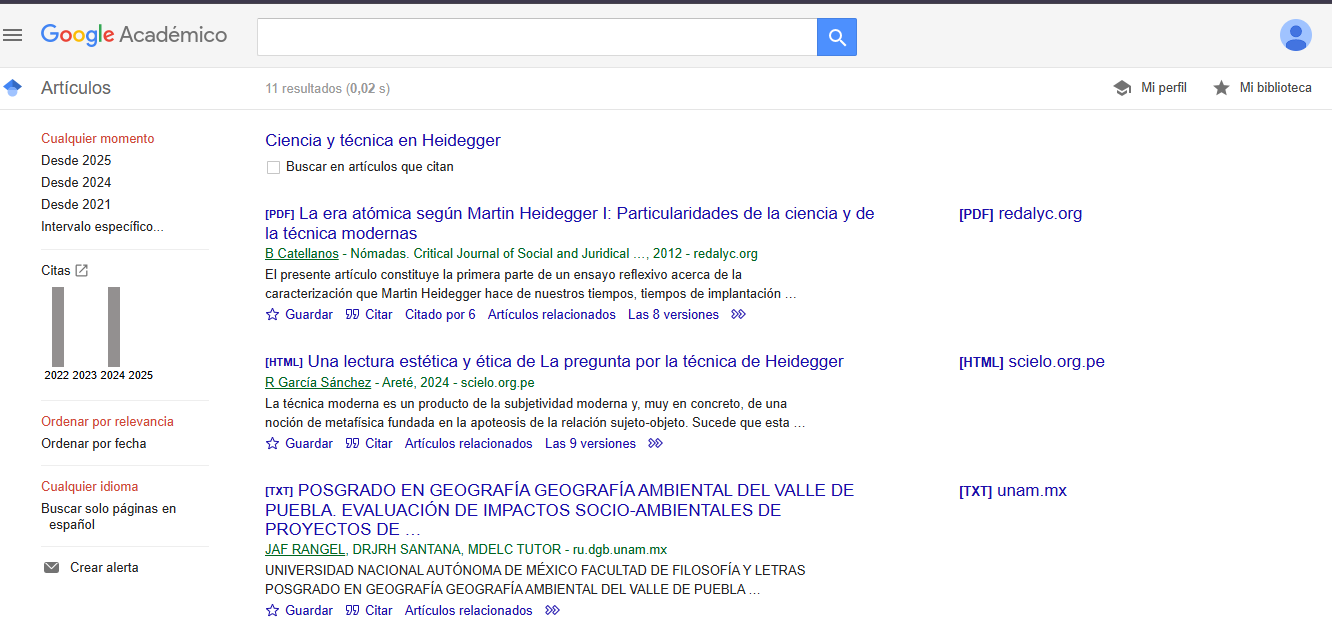
\includegraphics[width=0.8\linewidth]{heidegger citas.png}
    \label{}
\end{figure}
\begin{figure}[H]
    \centering
    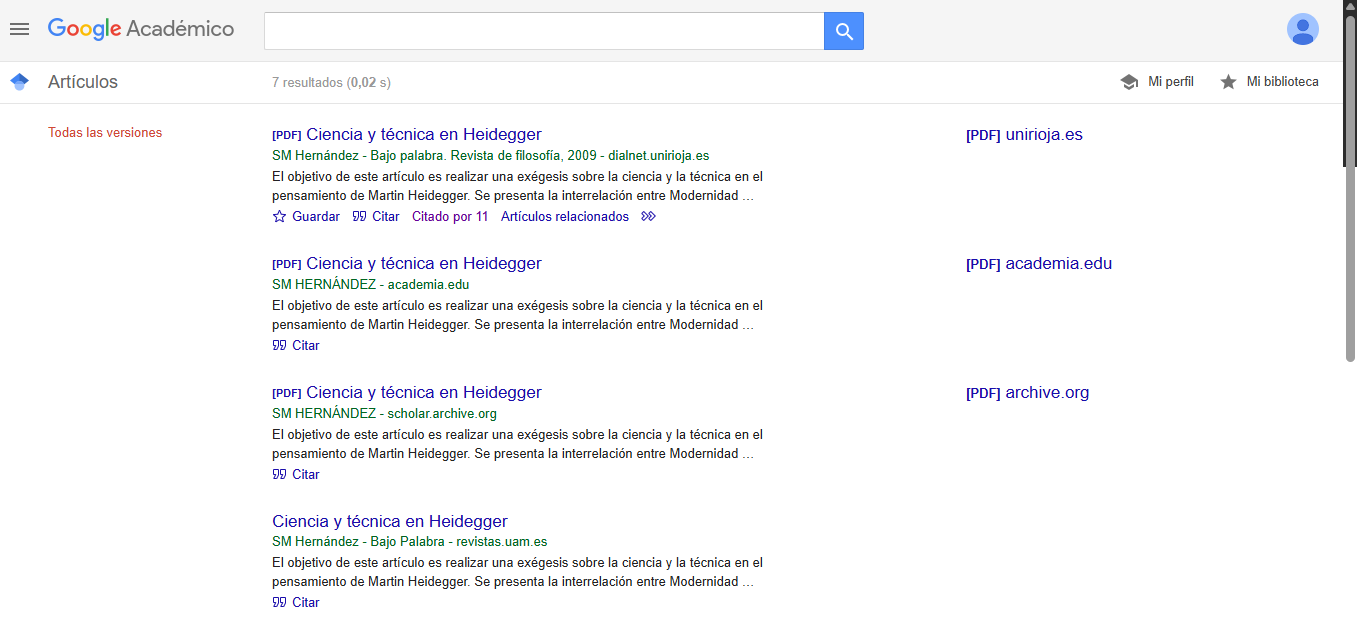
\includegraphics[width=0.8\linewidth]{Heidegger citas 2.png}
    \label{}
\end{figure}
Para el segundo artículo
\begin{figure}[H]
    \centering
    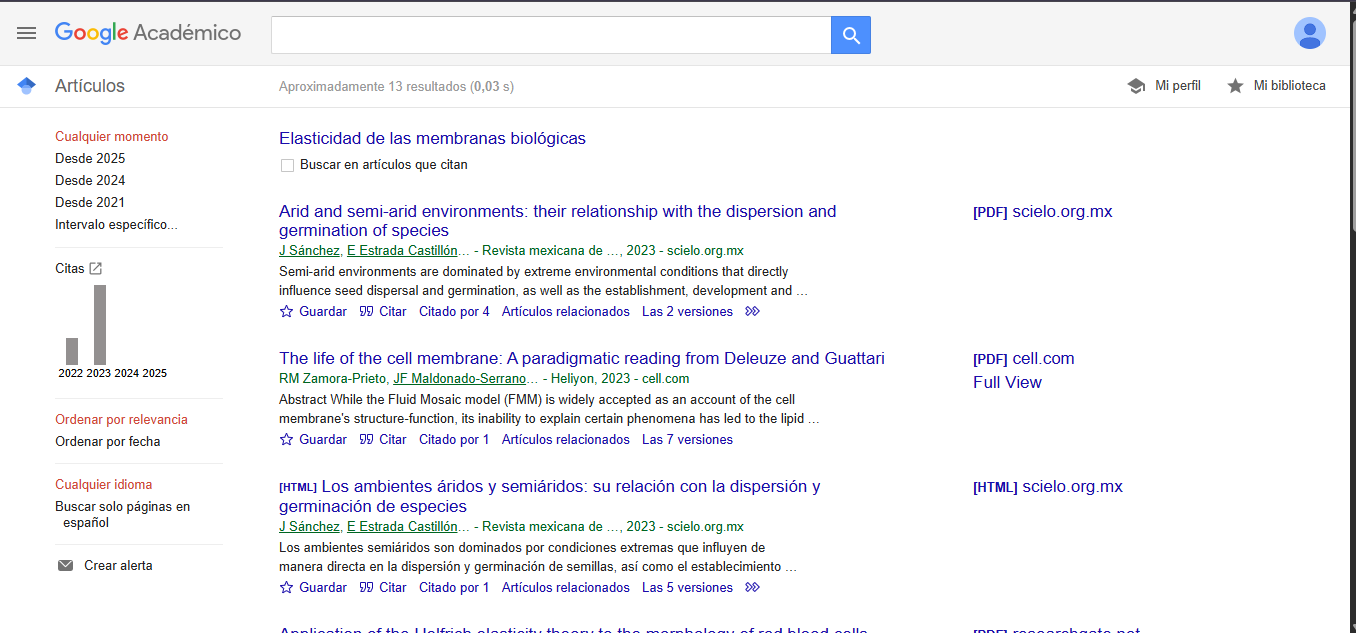
\includegraphics[width=0.8\linewidth]{biofisica citas.png}
    \label{}
\end{figure}
Posteriormente, volviendo a la página en la que encontramos el artículo, seleccionamos la opción de versiones para acceder a estas
Para el primer artículo se encontraron las siguientes versiones
\begin{figure}[H]
    \centering
    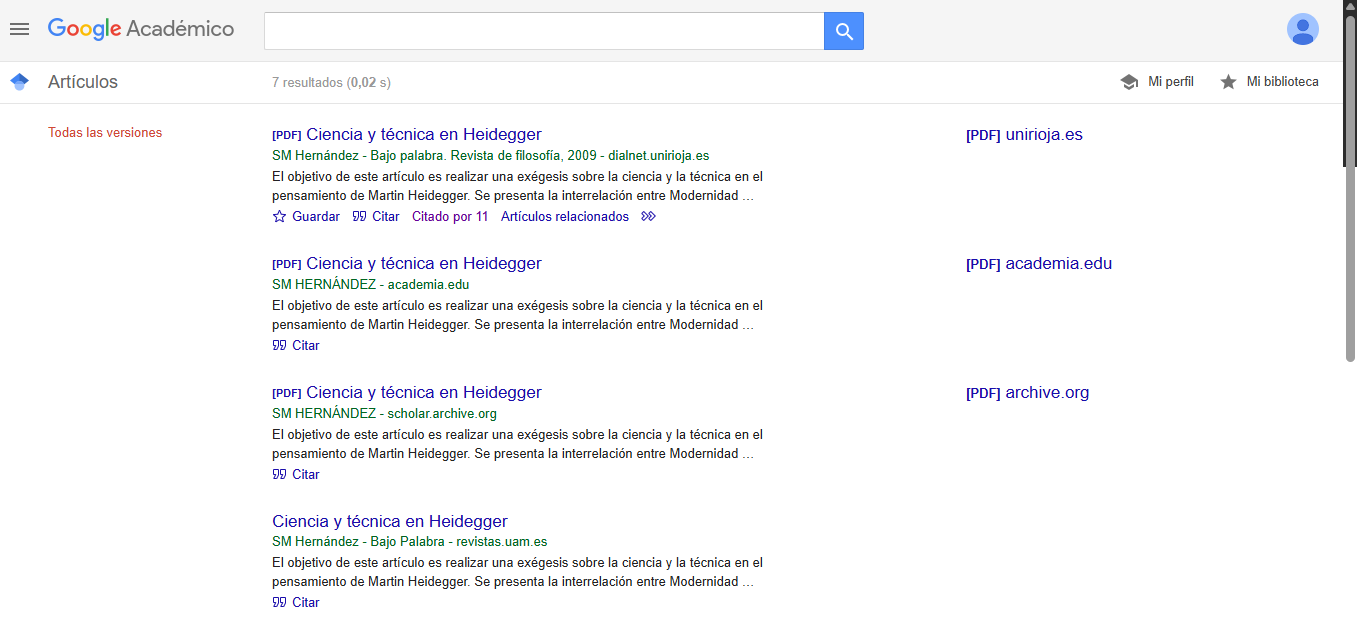
\includegraphics[width=0.8\linewidth]{heidegger versiones.png}
    \label{}
\end{figure}
\begin{figure}[H]
    \centering
    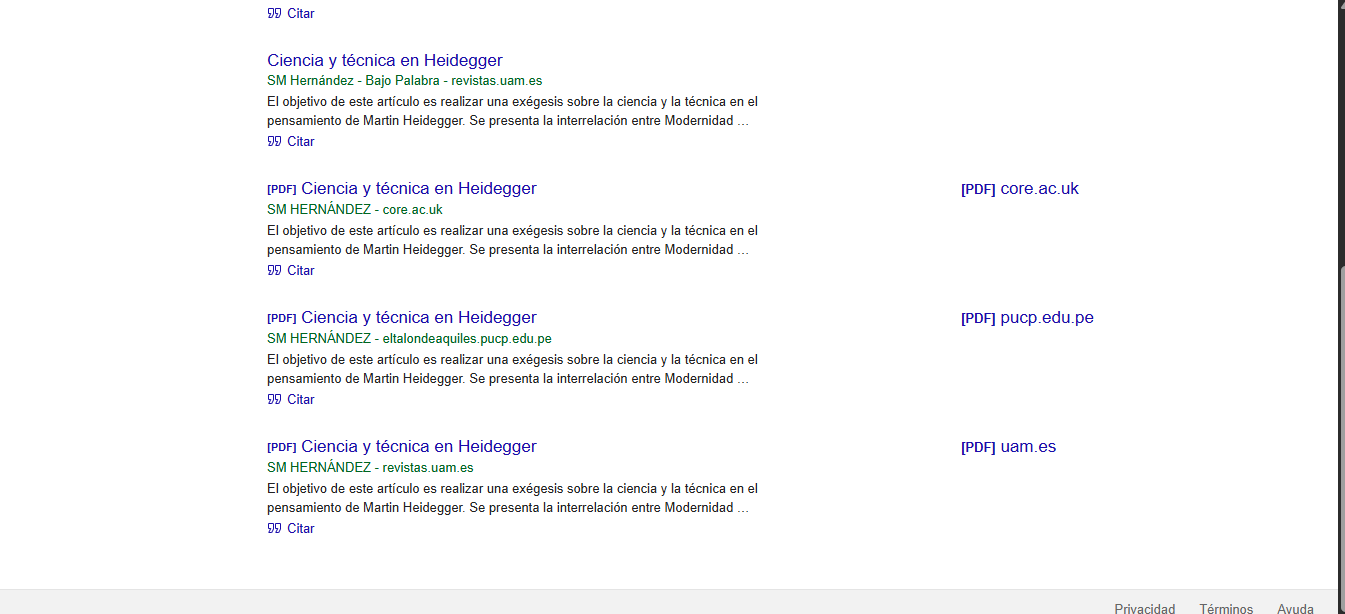
\includegraphics[width=0.8\linewidth]{heidegger versiones 2.png}
    \label{}
\end{figure}
Para el segundo artículo se encontraron las siguientes versiones
\begin{figure}[H]
    \centering
    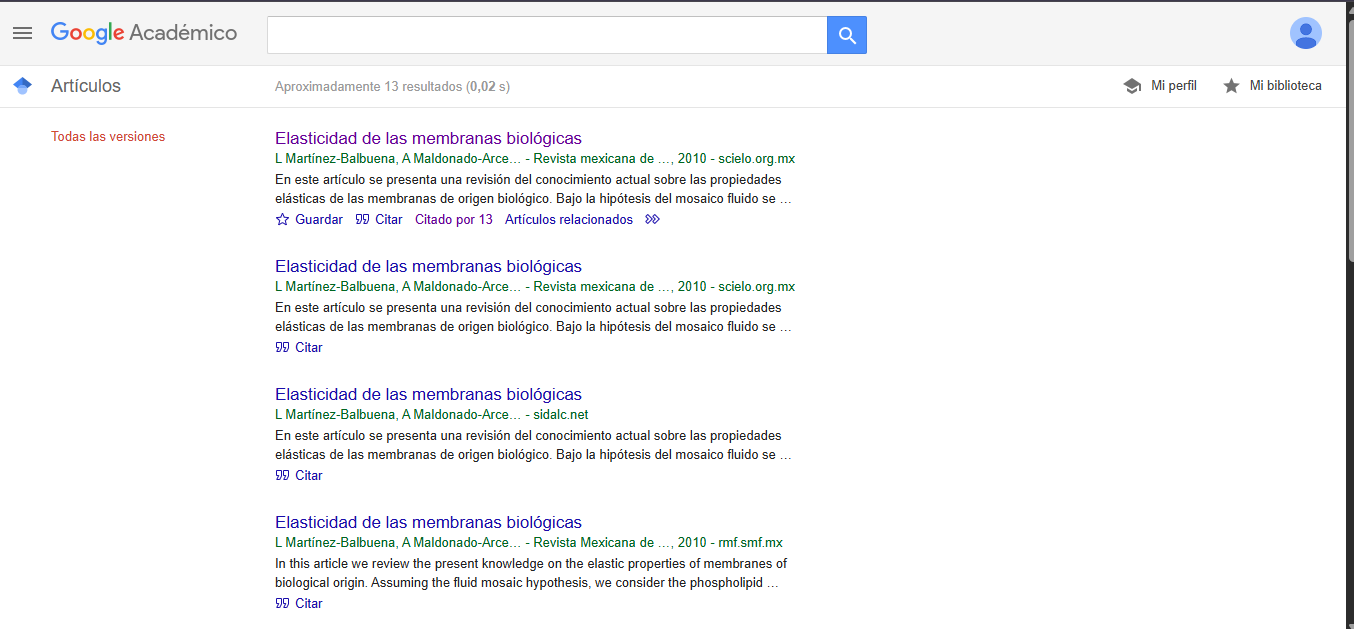
\includegraphics[width=0.8\linewidth]{biofisica versiones.png}
    \label{}
\end{figure}
\begin{figure}[H]
    \centering
    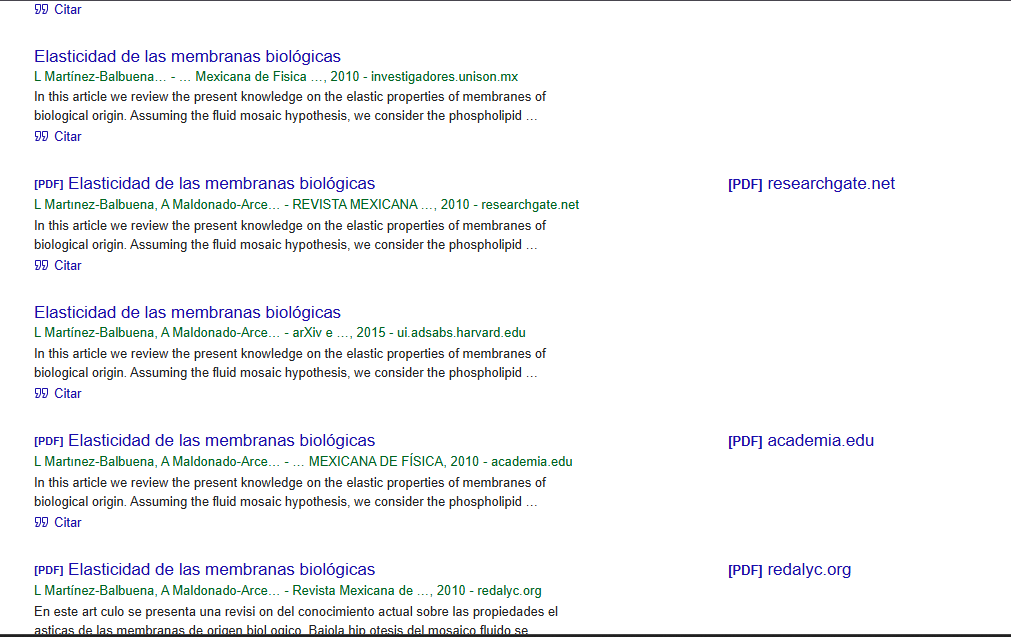
\includegraphics[width=0.8\linewidth]{biofisica versiones 2.png}
    \label{}
\end{figure}
\begin{figure}[H]
    \centering
    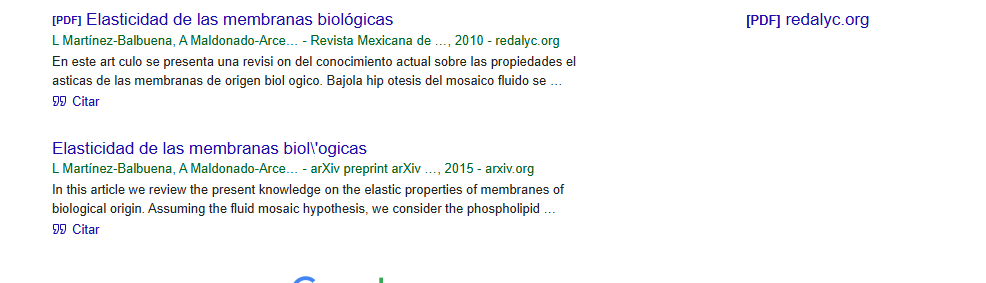
\includegraphics[width=0.8\linewidth]{biofisica versiones 3.png}
    \label{}
\end{figure}
A continuación se generaron alertas para ambos artículos
\begin{figure}[H]
    \centering
    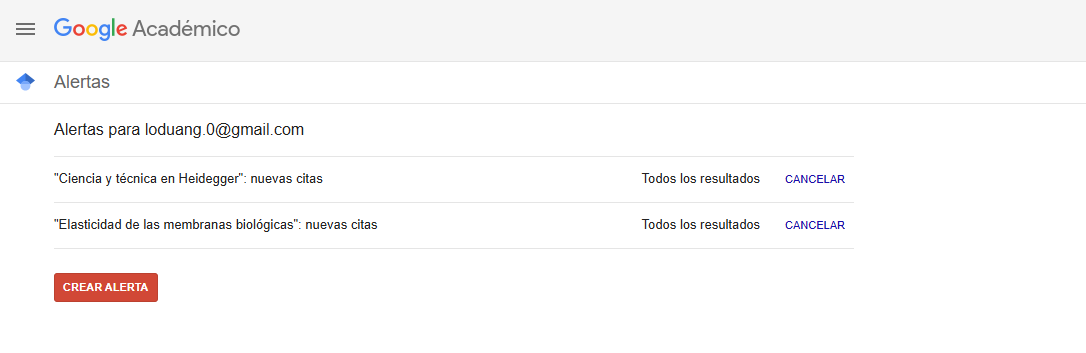
\includegraphics[width=0.8\linewidth]{crear alerta.png}
    \label{}
\end{figure}

Se desarrolló el mismo ejercicio utilizando Scinapsis

Primero se encontraron los artículos
\begin{figure}[H]
    \centering
    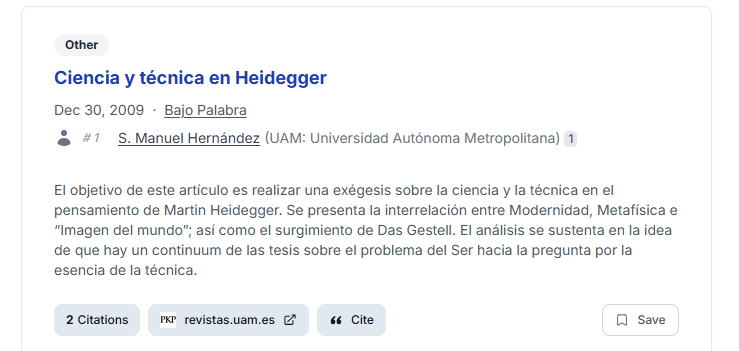
\includegraphics[width=0.8\linewidth]{scinapsis.png}
    \label{}
\end{figure}
\begin{figure}[H]
    \centering
    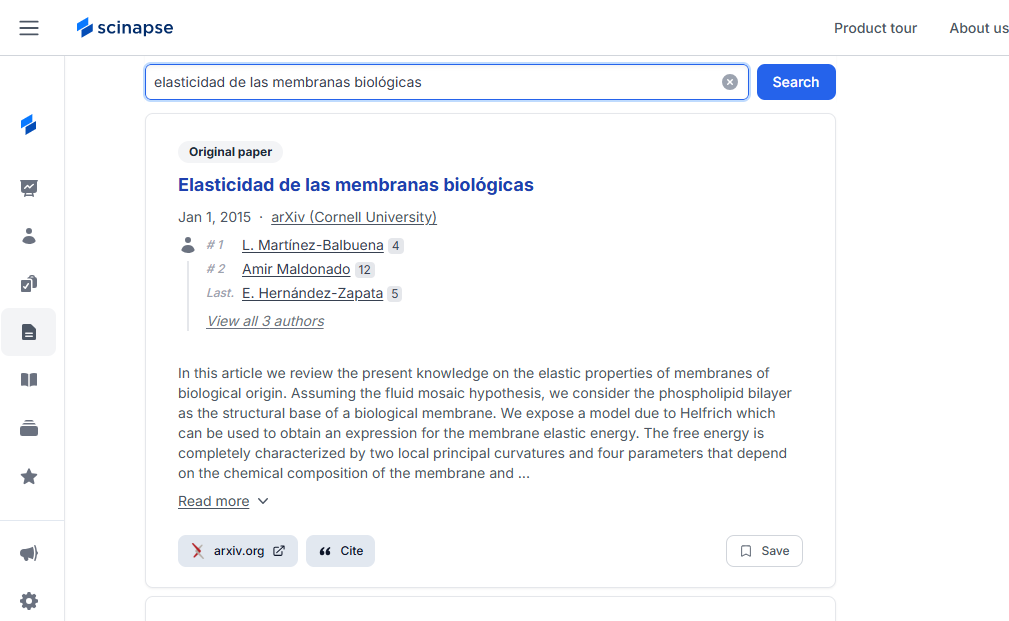
\includegraphics[width=0.8\linewidth]{scinapse bio.png}
    \label{}
\end{figure}

Luego, se buscaron los documentos en los que fueron citadas
\begin{figure}[H]
    \centering
    
\includegraphics[width=0.8\linewidth]{scinapsis citas.png}
    \label{}
\end{figure}
\begin{figure}[H]
    \centering
    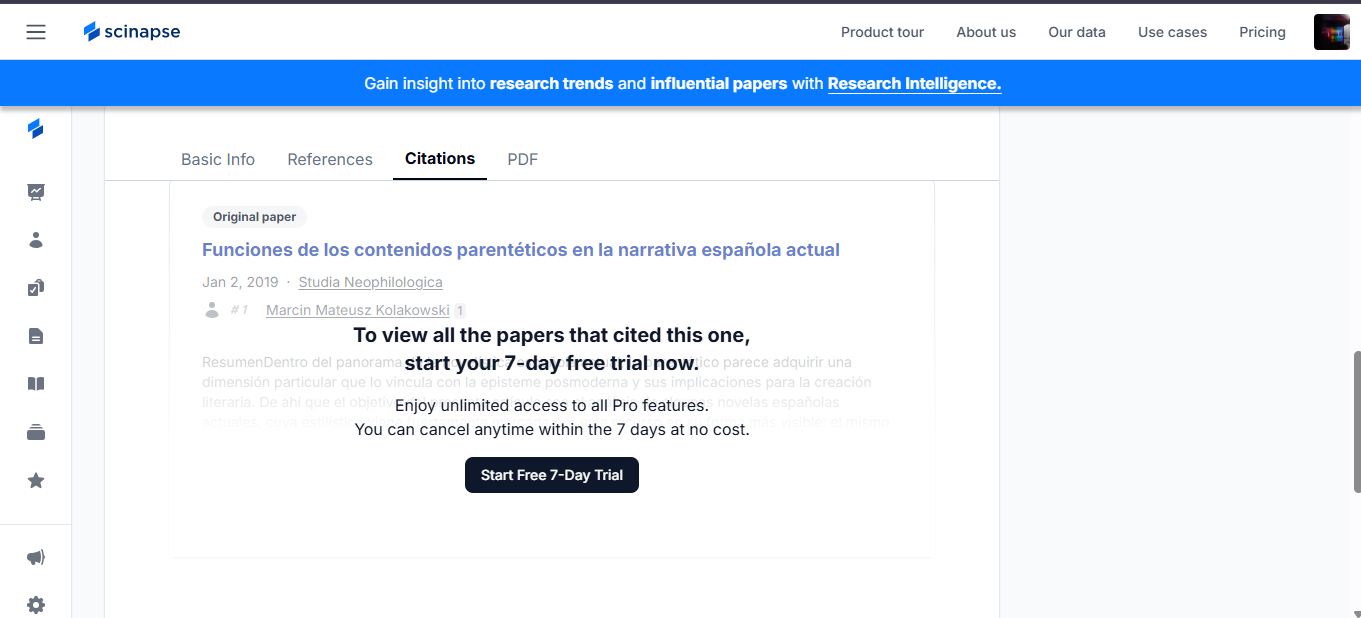
\includegraphics[width=0.8\linewidth]{scinapsis citas 2.png}
    \label{}
\end{figure}

Es evidente que, en contraste con Google Scholar, Scinapse no es gratuito, tiene menos información sobre las citas de estos artículos y solo cuenta con una versión de los mismos.


\section{}
\subsection{}

Lo primero que se debe hacer es ir \url{https://biblioteca.uniandes.edu.co}

bajando un poco encuentra la sección busqueda avanzada (Es un <a> tag de HTML con clase link, puede buscarlo con un scrapper con esta informacion). Tambien puedo decir que la URL que sostiene es \url{https://uniandes.primo.exlibrisgroup.com/discovery/search?vid=57U_UDLA:UDLA&lang=es&mode=advanced}. Dirigiendonos a esta pagina. Para buscar especificamente un trabajo de grado tenemos el siguiente menu:

\begin{figure}[H]
    \centering
    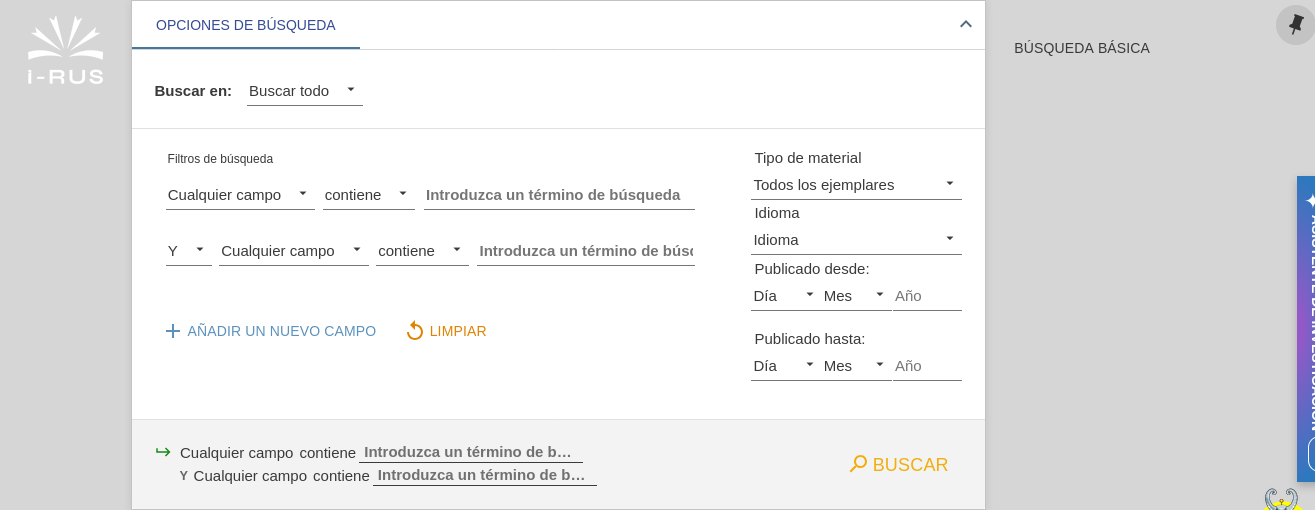
\includegraphics[width=0.8\linewidth]{Figures/section_2_a_p1.png}
    \label{fig:busqueda-avanzada}
\end{figure}

Como puede ver, lo que debe hacer es en la seccion de tipo de material al darle click le aparecera el siguiente menu:

\begin{figure}[H]
    \centering
    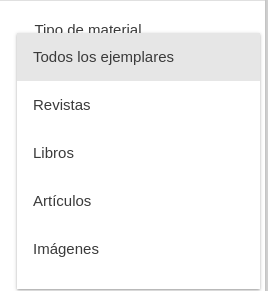
\includegraphics[width=0.8\linewidth]{Figures/section_2_a_p2.png}
    \label{fig:sec_2_a_p2}
\end{figure}

si baja al final de ese selector puede escoger trabajo de grado y proceder a buscar lo que quiera dandole click al boton buscar que puede encontrar en la figura \ref{fig:busqueda-avanzada}

Solo por diversion decidi hecharle un vistazo al como funcionaba este codigo y es simplemente un monton de parametros gets. Para este problema el importante es el parametro \textit{pfilter=rtype,exact,dissertations} el cual permite identificar que es lo que pasa. Por lo tanto para un scrapper lo mas facil es probablemente trabajar con estos strings para cambiar lo que se busca directamente.

\subsection{}

Divertamonos un poco con este punto...

Para iniciar tenemos muchisimas revistas para verlas puede ir a la pagina: \url{https://uniandes-co.libguides.com/az.php}

ahi puede encontrar cualquiera que desee. Busquemos entonces por ejemplo en science, proquest (computer science) y APS. Todas estas pueden ser simplemente encontradas buscandolas y si les da pereza son el unico resultado si pone estos links:
\begin{itemize}
    \item \url{https://uniandes-co.libguides.com/az.php?q=APS}
    \item \url{https://uniandes-co.libguides.com/az.php?q=proquest%20Computer%20Science}
    \item \url{https://uniandes-co.libguides.com/az.php?q=Science%20AAAS}
\end{itemize}

Simplemente le da click en el nombre. eso le abrira un mirror de la pagina pero pasando por un proxy de mo do que ahora tiene acceso a los contenidos. Ahora veamos como buscar:

\begin{figure}[H]
    \centering
    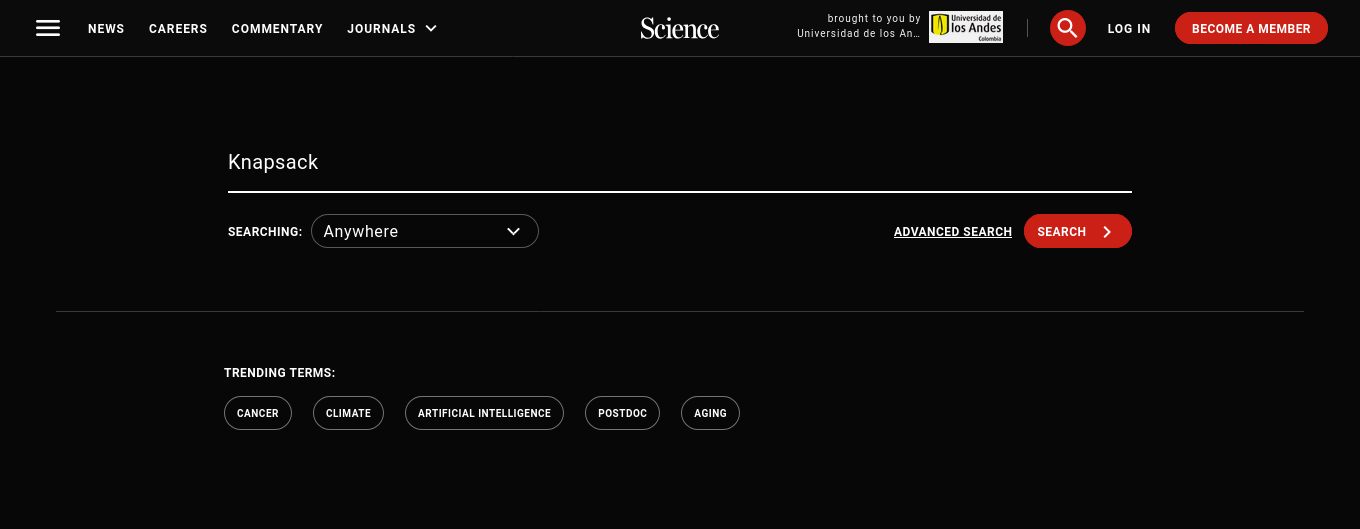
\includegraphics[width=0.8\linewidth]{Figures/section_2_b_p1.png}
    \label{fig:sec_2_b_p1}
\end{figure}

\begin{figure}[H]
    \centering
    
\includegraphics[width=0.8\linewidth]{Figures/section_2_b_p2.png}
    \label{fig:sec_2_b_p2}
\end{figure}

\begin{figure}[H]
    \centering
    
\includegraphics[width=0.8\linewidth]{Figures/section_2_b_p3.png}
    \label{fig:sec_2_b_p3}
\end{figure}

\section{}

Tras instalar Zotero como programa y como complemento para el navegador, se extrajo la información bibliográfica para el vídeo ''Feynman on scientific method'', el libro ''Naturalis Principia Mathematica´´ de Isaac Newton y el artículo ´´Gravitational Recoil and Suppression of Super Massive Black Hole Seeds in the Early Universe´´.

A continuación se muestra como se puede observar toda la información en el sistema Zotero

\begin{figure}[H]
    \centering
    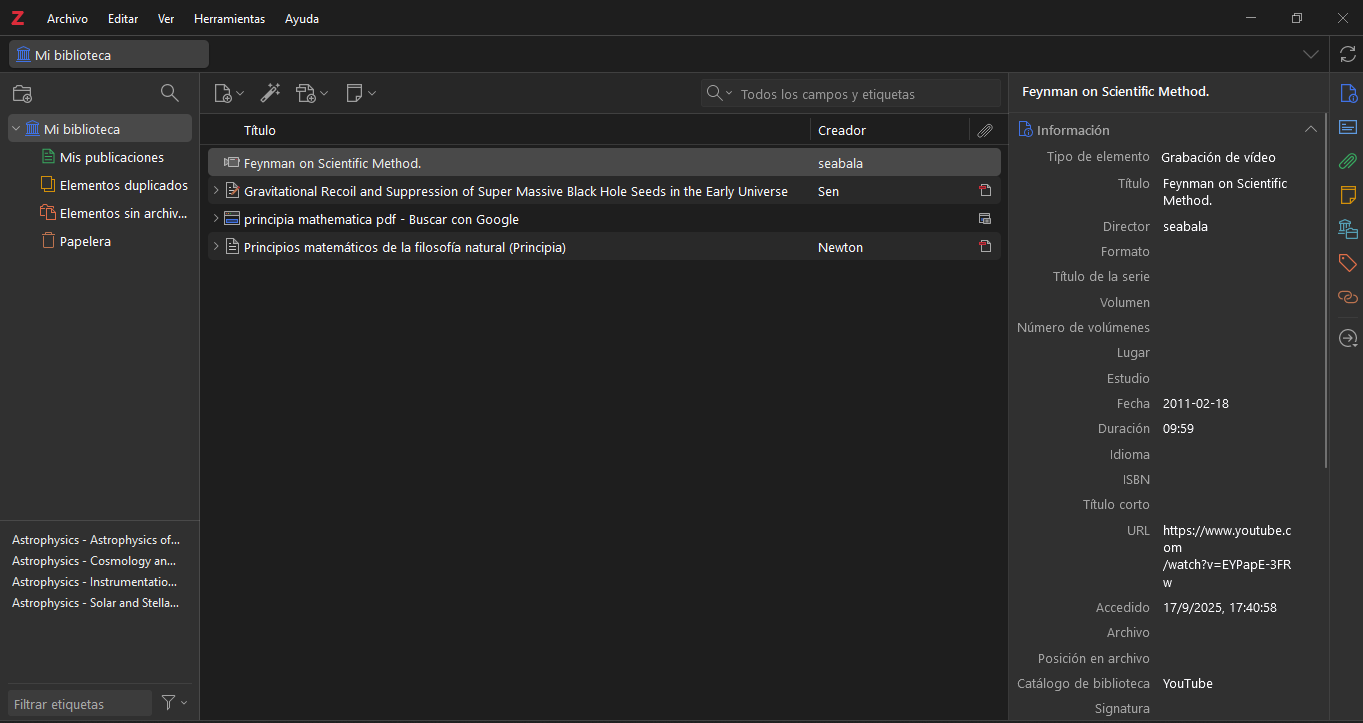
\includegraphics[width=0.8\linewidth]{Zotero 1.png}
    \label{}
\end{figure}
\begin{figure}[H]
    \centering
    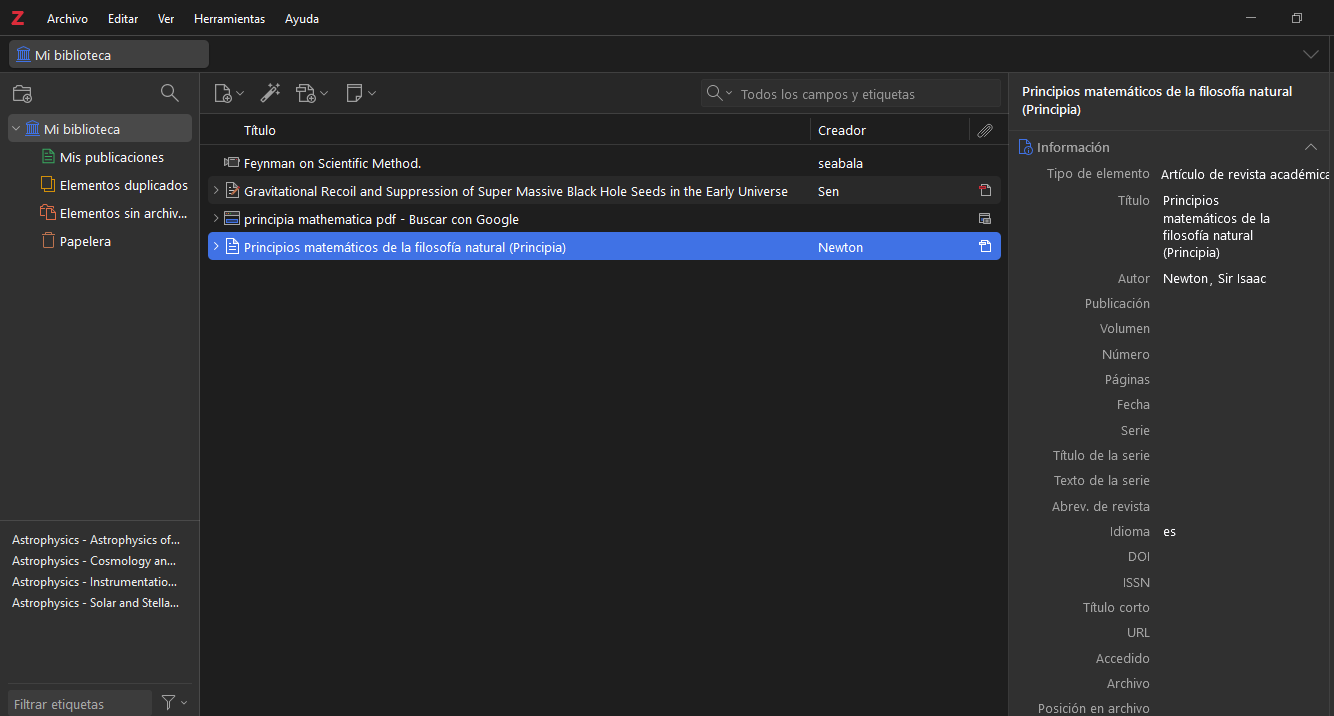
\includegraphics[width=0.8\linewidth]{Zotero libro.png}
    \label{}
\end{figure}
\begin{figure}[H]
    \centering
    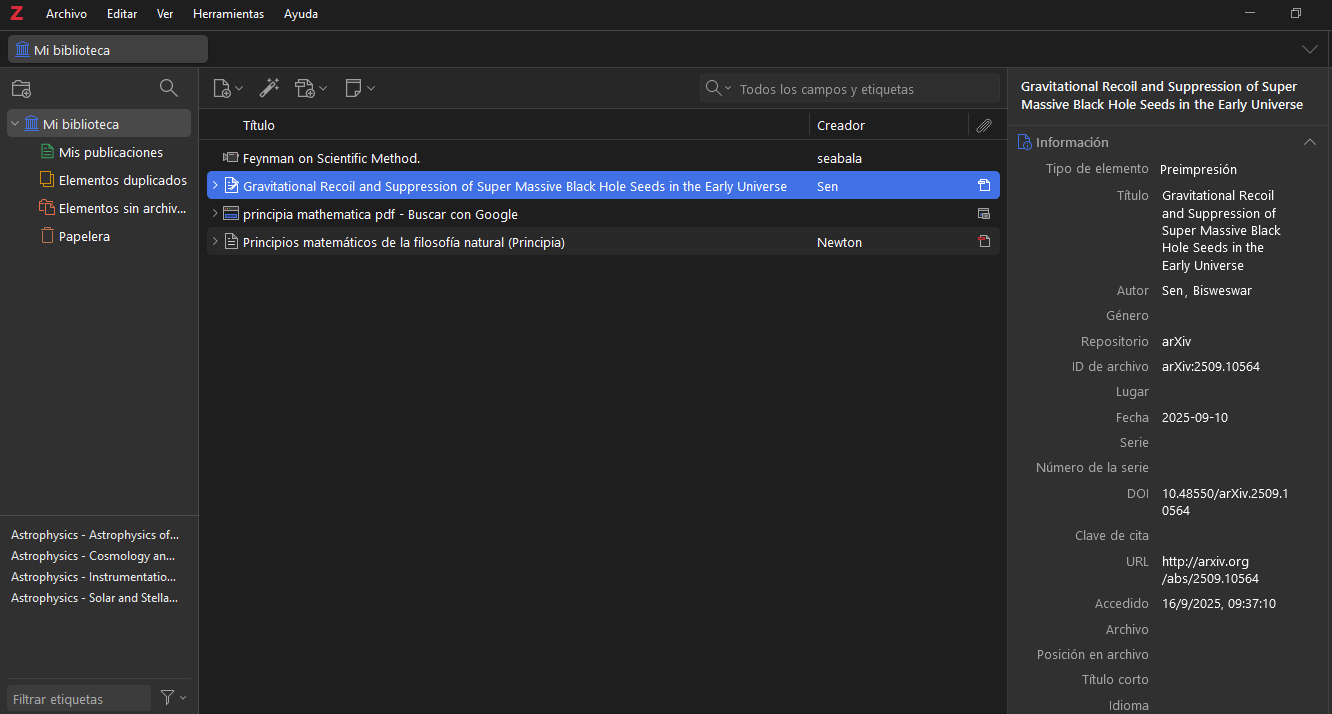
\includegraphics[width=0.8\linewidth]{zotero articulo.png}
    \label{}
\end{figure}

Posteriormente, se realizo una prueba para citar en estilo IEEE utilizando la herramienta de Zotero para Word en Google docs 

\begin{figure}[H]
    \centering
    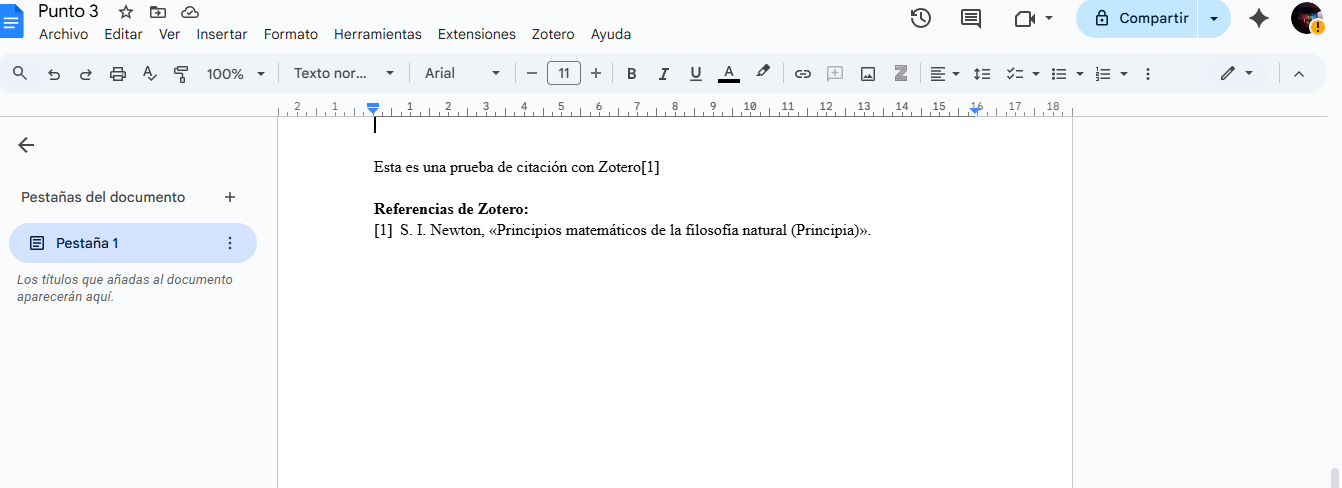
\includegraphics[width=0.8\linewidth]{word zotero.png}
    \label{}
\end{figure}

Finalmente, se generaron las referencias en BibtTex en Zotero y se genero el archivo .bib para cada caso (libro, artículo y vídeo) utilizando la opción exportar y seleccionando el tipo de aarchivo deseado

\begin{figure}[H]
    \centering
    
\includegraphics[width=0.8\linewidth]{Captura de pantalla 2025-09-17 205255.png}
    \label{}
\end{figure}

Con estos archivo, es posible citar en Latex como se muestra en esta prueba:
Para el artículo \cite{sen_gravitational_2025}
Para el video \cite{seabala_feynman_2011}
Para el libro \cite{newton_principios_nodate}




\section{}

\subsection{}

En este caso iniciamos desde Zotero y con una cita ya cargada. Podemos dar click derecho y nos sale lo siguiente:


\begin{figure}[H]
    \centering
    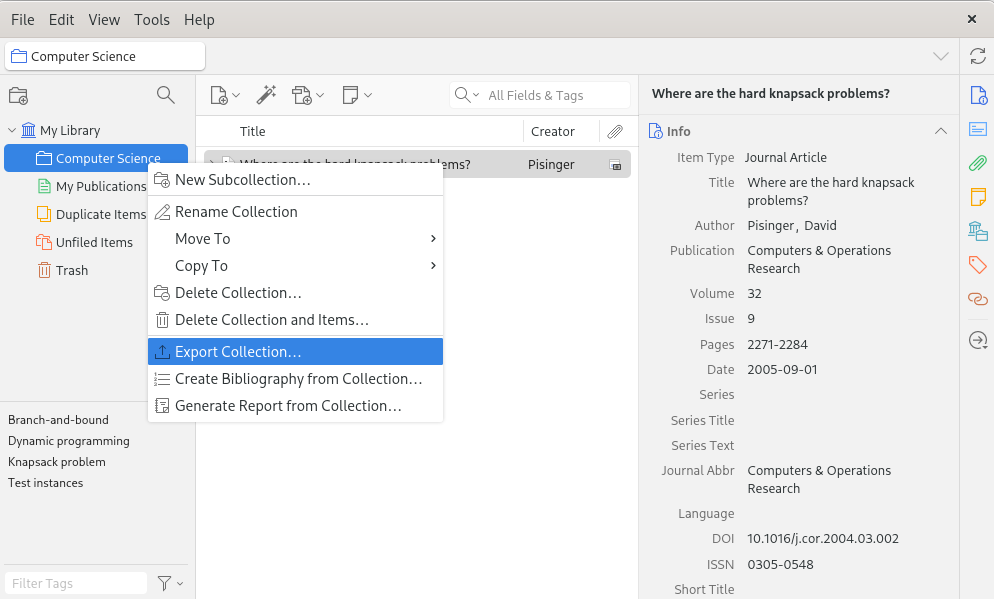
\includegraphics[width=0.8\linewidth]{Figures/section_4_a_p1.png}
    \label{fig:sec_4_a_p1}
\end{figure}

Escogiendo la opcion que aparece en la imagen (exportar) de ahi sale otro menu en donde debemos escoger bibtex (por que es lo que estamos usando, aunque bibLatex es probablemente una mejor opcion dado que estamos trabajando sobre compiladores modernos de \LaTeX no de \TeX{} ademas de que es un proyecto que es activamente mantenido).

Escoja tambien codificar en UTF-8. Es probablemente el mas estandar y el locale de su pc es lo mas probable que sea ese. Igual puede ser recomendable que lo cambie en caso de que este manejando una configuración particularmente obscura. 

Al final se debe ver algo asi:

\begin{figure}[H]
    \centering
    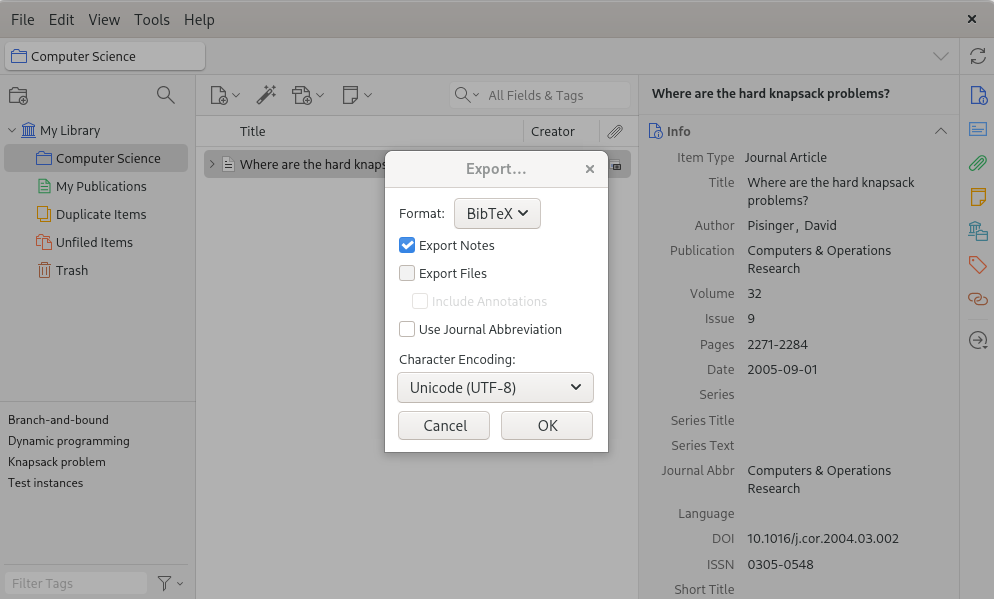
\includegraphics[width=0.8\linewidth]{Figures/section_4_a_p2.png}
    \label{fig:sec_4_a_p2}
\end{figure}

De click en Ok y lleve us archivo .bib a su proyecto. Esto es sumamente dependiente de la interfaz, yo estoy en un debian 13 con gnome para no complicarme y por tanto tengo que simplemente navegar nautilus pero su caso puede variar. 

Ahora bien, ya teniendo un bibtex configurado la conexion con latex es trivial y puramente codigo. Simplemente es usar el comando

\begin{verbatim}
\cite{<referencia>} %% uno cada vez que estes citando algo

\bibliographystyle{<Nombre del estilo>}

\bibliography{<Nombre de la sección>}
\end{verbatim}

\subsection{}

simplemente cambia el comando de arriba para el estilo que quieres:

\begin{verbatim}
\cite{<referencia>} %% uno cada vez que estes citando algo.

\bibliographystyle{prl} %% Hay un monton mas por cierto,
%% aunque es probable que lo mejor
%% sea que uses biblatex de nuevo.

\bibliography{<Nombre de la sección>}
\end{verbatim}

\subsection{}

Asumiendo que tu entrada de bibtex tiene una URL que en caso de que no es simplemente esto:
\begin{verbatim}
@<estilo>{<identificador>,
    ...
    % Simplmente agrega esta linea 
    url = {<url>}
    ...
}
\end{verbatim}

lo mas facil como estamos es usar el estilo \textit{apsrev4-1}. No nos compliquemos de mas.

\subsection{}

Esto es lo mismo que en el punto a de esta seccion. Ojo que no lo estoy diciendo en chiste. Conozco el plugin para conectar Overleaf con Zotero y puedo entender los argumentos de por que seria mejor. Sin embargo, \LaTeX es un lenguaje de programación (Bueno, usted gana es un conjunto de comandos y macros sobre el lenguaje de programacion que es \TeX) y como tal considero que es mejor mantenerlo asi. En el peor de los casos puede crear un pequeño script que actualice el bibtex cada vez que lo vaya a compilar y ejecutarlo junto con un Makefile. 

Me niego a considerar la manera \textit{correcta} seder mi libertad, dignidad y patromonio digital a una empresa.



\bibliographystyle{apalike}  
%\bibliography{referencias} 
\bibliography{artículo_bibtex, newton_bibtex, video_bibtex}

\end{document}
